\documentclass[12pt]{article}
\usepackage[utf8]{inputenc}
\usepackage{amsmath}
\usepackage{amssymb}
\usepackage{geometry}
\usepackage{graphicx}
\usepackage{hyperref}
\usepackage{physics}
\usepackage{caption}
\usepackage{subcaption}
\usepackage{enumitem}
\usepackage{titlesec}
\usepackage{float}
\usepackage[table]{xcolor}
\usepackage{colortbl}
\usepackage{array}
\usepackage{makecell}
\usepackage{listings}

\lstset{
	numbers=left,
	tabsize=1,
	tab=1,
	xleftmargin=1pt,
	basicstyle=\ttfamily,
	breaklines=true,
	frame=single,
}

\geometry{
	a4paper,
	left=25mm,
	right=25mm,
	top=25mm,
	bottom=25mm
}

\title{
	\textbf{Principles of Data Communications and Networks Modeling (CS4865/6865)} \\[2mm]
	\text{Lab Report \#2: Introduction to network simulation II}
}
\author{Abid Hasan Muin (3804634)}
\date{Due date: October 14, 2025}


\titleformat{\section}{\large\bfseries}{Exercise \thesection:}{1em}{}
\setcounter{section}{0}

\begin{document}
	
	\maketitle
	
	% Exercise 1
	\section{}
	
	% Exercise 1.1
	\subsection{UDP data flow example}
	
	\begin{figure}[htbp]
		\centering
		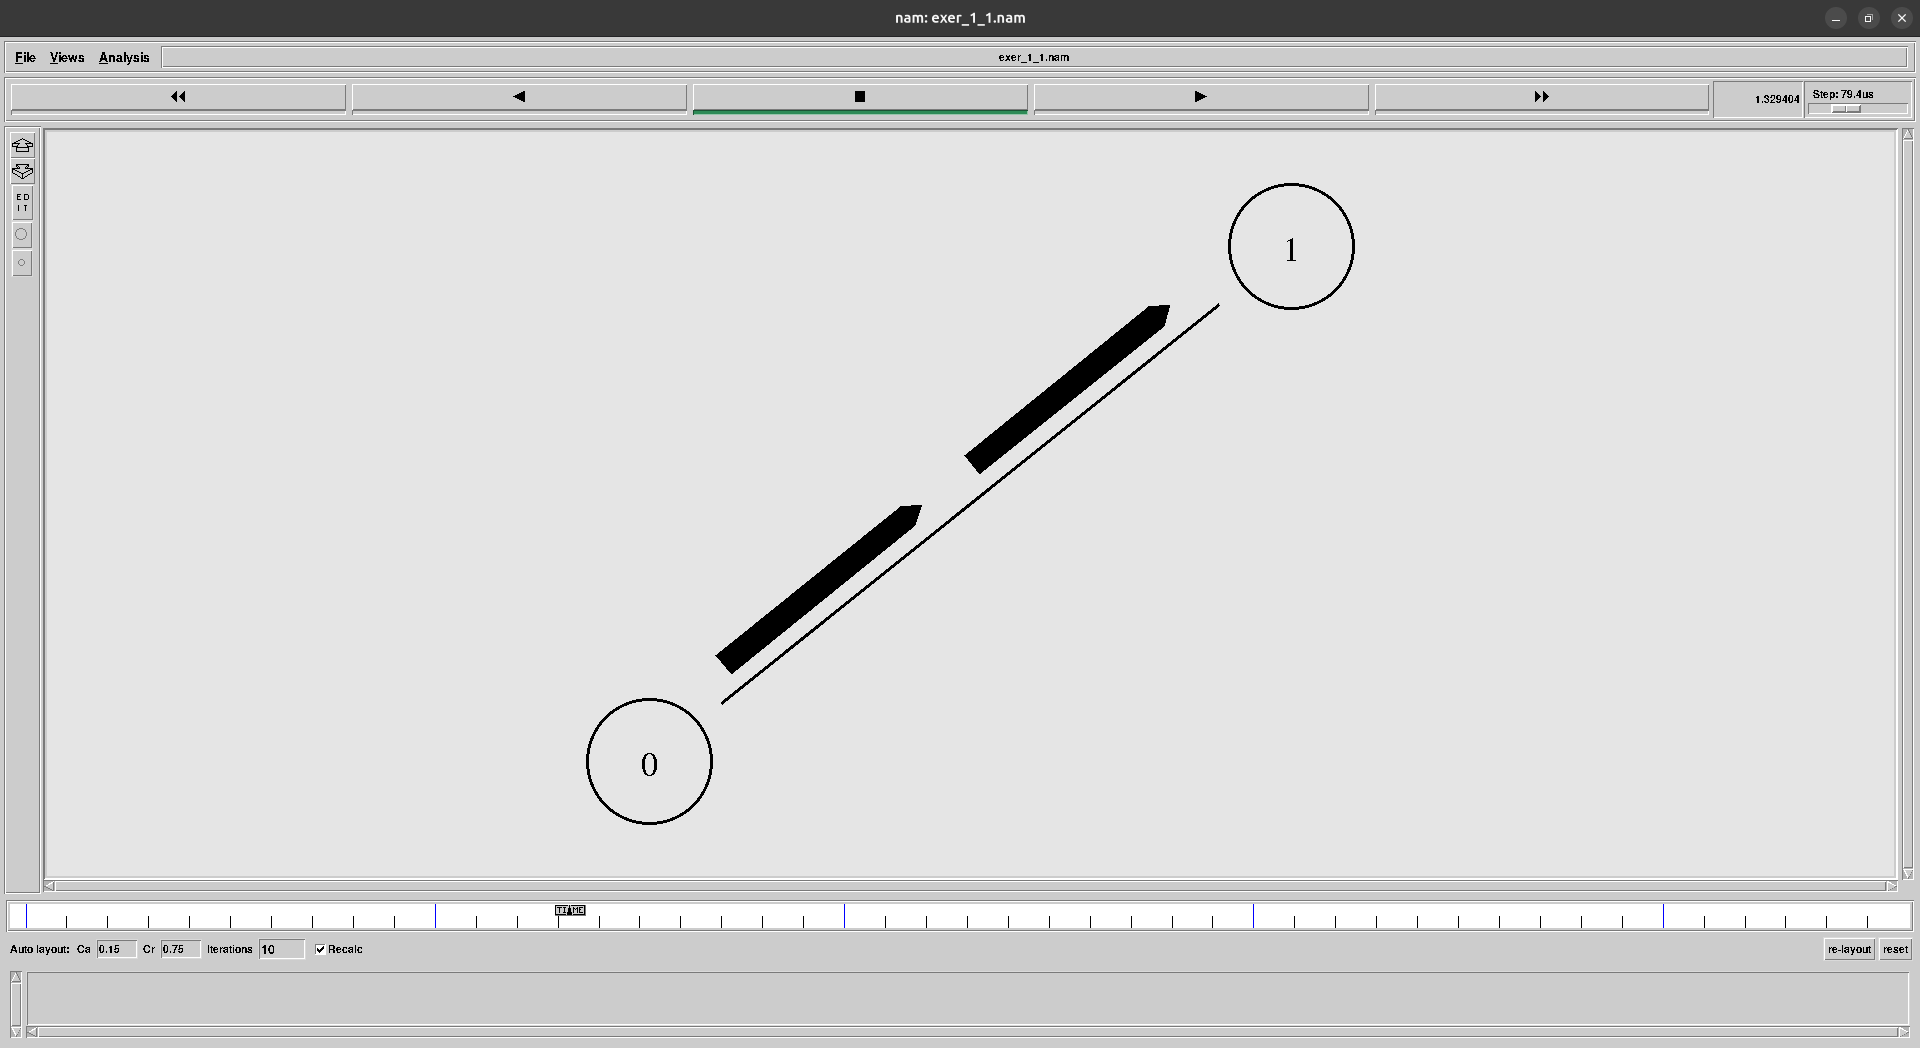
\includegraphics[width=\textwidth]{exer_1_1.png}
		\caption{UDP data flow example}
		\label{fig:exer_1_1}
	\end{figure}
	
	% Exercise 1.2
	\subsection{Throughput Calculation}
	
	From the trace file, we get: \\
	\\
	Timestamp of first packet (send) = 0.5 \\
	Timestamp of last packet (received) = 4.51 \\
	Total duration of transfer = (4.51 - 0.5) = 4.01 \\
	\\
	Total packets transferred = 801 \\
	Size of each packet = 500 bytes \\
	Total data transferred = $801\times500\times8$ = 3,204,000 bits
	\\
	Effective throughput = $\frac{3,204,000}{4.1}~\mathrm{bps}$ $\approx$ 781,463.41 bps $\approx$ 781.46 kbps
	\\
	\noindent
	\textbf{Relevant trace file line:}
	\begin{lstlisting}
	+ -t 0.5 -s 0 -d 1 -p cbr -e 500 -c 0 -i 0 -a 0 -x {0.0 1.0 0 ------- null}
	r -t 4.51399999999993 -s 0 -d 1 -p cbr -e 500 -c 0 -i 800 -a 0 -x {0.0 1.0 800 ------- null}
	\end{lstlisting}
	
	% Exercise 1.3
	\subsection{Throughput value comparison}
	From the \textit{.tcl} file, we get: \\
	\\
	Packet size = 500 bytes = 4000 bits \\
	Packet send interval = 0.005 seconds \\
	Theoretical throughput = $\frac{4000}{0.005}~\mathrm{bps}$ = 800,000 bps = 800 kbps\\
	\\
	\textbf{Comparison:} \\
	Theoretical throughput = 800 kbps \\
	Effective throughput = 781.46 kbps
	
	 
	% Exercise 2
	\section{}
	
	% Exercise 2.1
	\subsection{Stop and Wait TCP Flow}
	
	The main difference is that in Exercise 2.1 (TCP with window = 1), the traffic behaves like a stop-and-wait protocol which means only one packet is sent at a time, and the sender waits for an acknowledgment before sending the next. In contrast, the UDP/CBR flow in Exercise 1.1 sends packets continuously and quickly, regardless of acknowledgments.
	
	\begin{figure}[H]
		\centering
		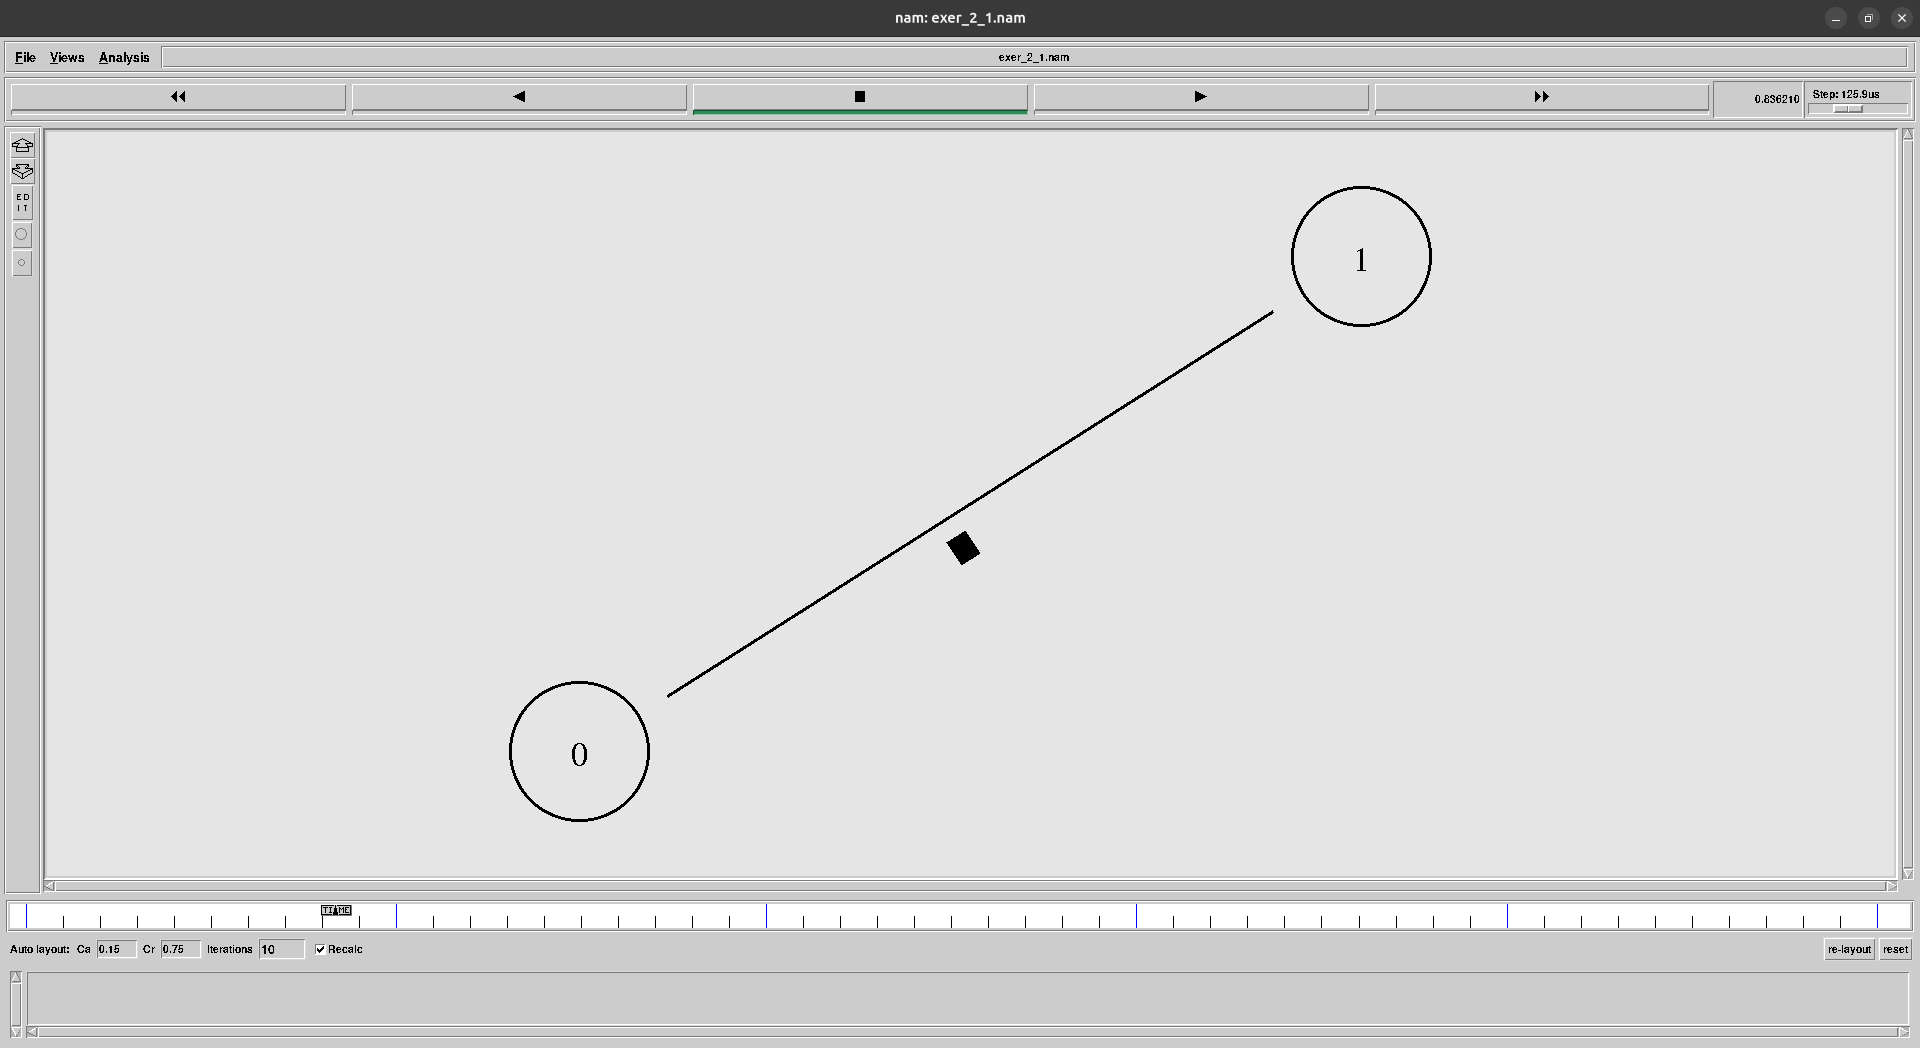
\includegraphics[width=\textwidth]{exer_2_1.png}
		\caption{Stop and Wait TCP flow example}
		\label{fig:exer_2_1}
	\end{figure}
	
	\noindent
	\textbf{Source code:}
	\begin{lstlisting}
	# Create a simulator object
	set ns [new Simulator]
	
	# Open the nam trace file
	set nf [open exer_2_1.nam w]
	$ns namtrace-all $nf
	
	# Define a 'finish' procedure
	proc finish {} {
		global ns nf
		$ns flush-trace
		close $nf
		exec nam exer_2_1.nam &
		exit 0
	}
	
	# Create two nodes
	set n0 [$ns node]
	set n1 [$ns node]
	
	# Create a duplex link between the nodes
	$ns duplex-link $n0 $n1 1Mb 10ms DropTail
	
	# Create a TCP agent and attach it to node n0
	set tcp0 [new Agent/TCP]
	$tcp0 set packetSize_ 500         ;# Set packet size to 500
	$tcp0 set window_ 1               ;# Set max window size to 1
	$ns attach-agent $n0 $tcp0
	
	# Create a TCP Sink agent and attach it to node n1
	set sink0 [new Agent/TCPSink]
	$ns attach-agent $n1 $sink0
	
	# Connect the TCP agent to the sink
	$ns connect $tcp0 $sink0
	
	# Create an FTP application and attach it to the TCP agent
	set ftp0 [new Application/FTP]
	$ftp0 attach-agent $tcp0
	
	# Start the FTP traffic at 0.5s
	$ns at 0.5 "$ftp0 start"
	
	# Call the finish procedure at 5.0s
	$ns at 5.0 "finish"
	
	# Run the simulation
	$ns run
	\end{lstlisting}
	
	% Exercise 2.2
	\subsection{Throughput Calculation}
	Since TCP connection has network overhead, I have only considered the actual payload or data that was transferred. \\
	From the trace file, we get: \\
	\\
	Timestamp of first packet (send) = 0.52 \\
	Timestamp of last packet (received) = 4.99 \\
	Total duration of transfer = (4.99 - 0.52) = 4.47 \\
	\\
	Total packets transferred = 182 \\
	Size of each packet = 500 bytes \\
	Total data transferred = $182\times500\times8$ = 728,000 bits
	\\
	Effective throughput = $\frac{728,000}{4.47}~\mathrm{bps}$ $\approx$ 162,863.53 bps $\approx$ 162.86 kbps
	\\
	\noindent
	\textbf{Relevant trace file line:}
	\begin{lstlisting}
	+ -t 0.52064 -s 0 -d 1 -p tcp -e 540 -c 0 -i 2 -a 0 -x {0.0 1.0 1 ------- null}
	r -t 4.99480000000002 -s 0 -d 1 -p tcp -e 540 -c 0 -i 364 -a 0 -x {0.0 1.0 182 ------- null}
	\end{lstlisting}
	
	% Exercise 2.3
	
	\subsection{Throughput value comparison}
	From the \textit{.tcl} file, we get: \\
	For Link (n0-n1): \\
	Bandwidth (Data Rate): 1Mb = 1 Mbps \\
	Delay = 10ms (one-way) \\
	\\
	\noindent
	ForTCP Agent: \\
	Packet Size: 500 bytes \\
	Window Size: 1 packet \\
	\\
	\noindent
	\textbf{Throughput Calculation:} \\
	RTT = 2 $\times$ 10 ms = 20 ms \\
	Theoretical throughput = $\frac{4000\times1}{0.02}~\mathrm{bps}$ = 200,000 bps = 200 kbps\\
	\\
	\textbf{Comparison:} \\
	Theoretical throughput = 200 kbps \\
	Effective throughput = 162.86 kbps
	
	% Exercise 3
	\section{}
	
	% Exercise 3.1
	\subsection{Stop and Wait TCP Flow}
	
	By increasing the TCP window size from 1 to 2, the sender can transmit two packets before waiting for acknowledgments, instead of just one. This improves throughput and link utilization by reducing idle time between packet transmissions.
	
	\begin{figure}[H]
		\centering
		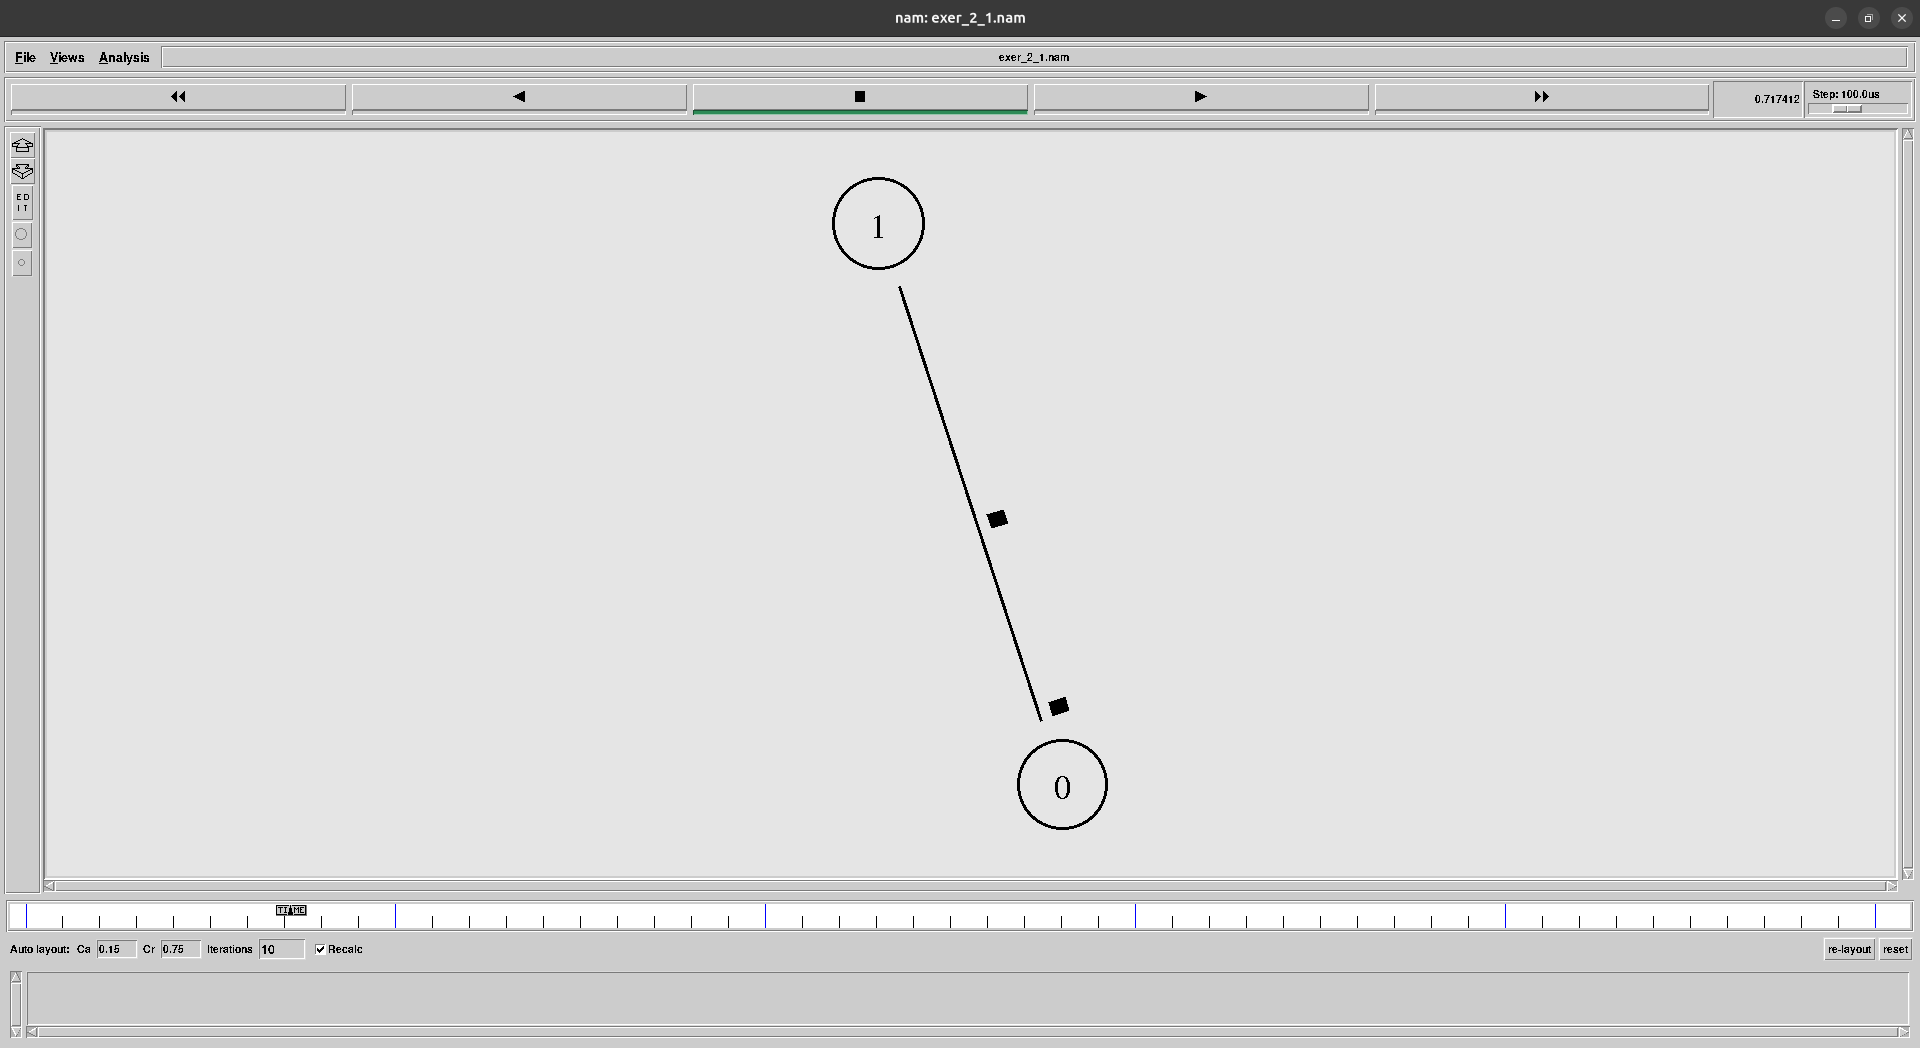
\includegraphics[width=\textwidth]{exer_3_1.png}
		\caption{Stop and Wait TCP flow example}
		\label{fig:exer_3_1}
	\end{figure}
	
	\noindent
	\textbf{Source code:}
	\begin{lstlisting}
	# Create a simulator object
	set ns [new Simulator]
	
	# Open the nam trace file
	set nf [open exer_3_1.nam w]
	$ns namtrace-all $nf
	
	# Define a 'finish' procedure
	proc finish {} {
		global ns nf
		$ns flush-trace
		close $nf
		exec nam exer_3_1.nam &
		exit 0
	}
	
	# Create two nodes
	set n0 [$ns node]
	set n1 [$ns node]
	
	# Create a duplex link between the nodes
	$ns duplex-link $n0 $n1 1Mb 10ms DropTail
	
	# Create a TCP agent and attach it to node n0
	set tcp0 [new Agent/TCP]
	$tcp0 set packetSize_ 500         ;# Set packet size to 500
	$tcp0 set window_ 2               ;# Set max window size to 2
	$ns attach-agent $n0 $tcp0
	
	# Create a TCP Sink agent and attach it to node n1
	set sink0 [new Agent/TCPSink]
	$ns attach-agent $n1 $sink0
	
	# Connect the TCP agent to the sink
	$ns connect $tcp0 $sink0
	
	# Create an FTP application and attach it to the TCP agent
	set ftp0 [new Application/FTP]
	$ftp0 attach-agent $tcp0
	
	# Start the FTP traffic at 0.5s
	$ns at 0.5 "$ftp0 start"
	
	# Call the finish procedure at 5.0s
	$ns at 5.0 "finish"
	
	# Run the simulation
	$ns run
	\end{lstlisting}
	
	% Exercise 3.2
	\subsection{Throughput Calculation}
	Since TCP connection has network overhead, I have only considered the actual payload or data that was transferred. \\
	From the trace file, we get: \\
	\\
	Timestamp of first packet (send) = 0.52 \\
	Timestamp of last packet (received) = 4.99 \\
	Total duration of transfer = (4.99 - 0.52) = 4.47 \\
	\\
	Total packets transferred = 364 \\
	Size of each packet = 500 bytes \\
	Total data transferred = $364\times500\times8$ = 1,456,000 bits
	\\
	Effective throughput = $\frac{1,456,000}{4.47}~\mathrm{bps}$ $\approx$ 325,727.07 bps $\approx$ 325.73 kbps
	\\
	\noindent
	\\
	\textbf{Relevant trace file line:}
	\begin{lstlisting}
	+ -t 0.52064 -s 0 -d 1 -p tcp -e 540 -c 0 -i 2 -a 0 -x {0.0 1.0 1 ------- null}
	r -t 4.99912000000002 -s 0 -d 1 -p tcp -e 540 -c 0 -i 727 -a 0 -x {0.0 1.0 364 ------- null}
	\end{lstlisting}
	
	% Exercise 3.3
	
	\subsection{Throughput value comparison}
	From the \textit{.tcl} file, we get: \\
	For Link (n0-n1): \\
	Bandwidth (Data Rate): 1Mb = 1 Mbps \\
	Delay = 10ms (one-way) \\
	\\
	\noindent
	ForTCP Agent: \\
	Packet Size: 500 bytes \\
	Window Size: 2 packets \\
	\\
	\noindent
	\textbf{Throughput Calculation:} \\
	RTT = 2 $\times$ 10 ms = 20 ms \\
	Theoretical throughput = $\frac{4000\times2}{0.02}~\mathrm{bps}$ = 400,000 bps = 400 kbps\\
	\\
	\textbf{Comparison:} \\
	Theoretical throughput = 400 kbps \\
	Effective throughput = 325.73 kbps
	
	
	% Exercise 4
	\section{}
	
	% Exercise 4.1
	\subsection{Calculations for the interval parameter}
	
	For CBR traffic over UDP, the throughput is determined by: \\
	
	\begin{equation*}
		\text{Throughput (bps)} = \frac{\text{Packet Size (bytes)} \times 8}{\text{Interval (seconds)}}
	\end{equation*}

	\noindent
	For desired interval:
	\begin{equation*}
		\text{Interval} = \frac{\text{Packet Size (bytes)} \times 8}{\text{Desired Throughput}}
	\end{equation*}

	\noindent
	From the \textit{.tcl} script: \\
	Packet size = 500 bytes \\
	Desired throughput = 200 kbps = 200,000 bps
	
	\begin{equation*}
		\text{Interval} = \frac{500 \times 8}{\text{200,000}} = 0.02~\mathrm{seconds}
	\end{equation*}

	
	% Exercise 4.2
	\subsection{Throughput Calculation}
	From the trace file, we get: \\
	\\
	Timestamp of first packet (send) = 0.5 \\
	Timestamp of last packet (received) = 4.51 \\
	Total duration of transfer = (4.51 - 0.5) = 4.01 \\
	\\
	Total packets transferred = 200 \\
	Size of each packet = 500 bytes \\
	Total data transferred = $200\times500\times8$ = 800,000 bits
	\\
	Effective throughput = $\frac{800,000}{4.01}~\mathrm{bps}$ $\approx$ 199,501.25 bps $\approx$ 199.50 kbps
	\\
	\noindent
	\\
	\textbf{Relevant trace file line:}
	\begin{lstlisting}
		+ -t 0.5 -s 0 -d 1 -p cbr -e 500 -c 0 -i 0 -a 0 -x {0.0 1.0 0 ------- null}
		r -t 4.51399999999999 -s 0 -d 1 -p cbr -e 500 -c 0 -i 200 -a 0 -x {0.0 1.0 200 ------- null}
	\end{lstlisting}
	
	% Exercise 4.3
	
	\subsection{Achieved Link Utilization}
	
	\begin{equation*}
	Link Utilization (\%)=\frac{Throughput}{Link\ Capacity}\times~100
	\end{equation*}
	\noindent
	From the trace file: \\
	Link capacity = 1 Mbps = 1,000 kbps \\
	
	\textbf{For exercise 1:}
	\begin{equation*}
		Link Utilization (\%)=\frac{781.46}{1000}\times~100 \approx 7.81\%
	\end{equation*}
	
	\textbf{For exercise 2:}
	\begin{equation*}
		Link Utilization (\%)=\frac{162.86}{1000}\times~100 \approx 16.27\%
	\end{equation*}
	
	\textbf{For exercise 3:}
	\begin{equation*}
		Link Utilization (\%)=\frac{781.46}{1000}\times~100 \approx 32.57\%
	\end{equation*}
	
	\textbf{For exercise 4:}
	\begin{equation*}
		Link Utilization (\%)=\frac{199.5}{1000}\times~100 \approx 19.95\%
	\end{equation*}
	
	\noindent
	\textbf{Comment on link utilizations:}
	\begin{itemize}
		\item UDP can send faster, but without congestion control, it may lose packets, especially with DropTail.
		\item TCP is more reliable, but performance heavily depends on window size and round-trip time.
		\item Larger TCP window sizes significantly improve link utilization.
		\item Lower CBR rates result in underutilized links, while higher rates improve utilization but risk packet loss.
	\end{itemize}
	
	
	
	\begin{thebibliography}{9}
		\bibitem{mark} Mark Greis, Tutorial for the Network Simulator "ns": \url{http://www.isi.edu/nsnam/ns/tutorial/index.html}
		\bibitem{tcl} TCL description: \url{http://en.wikipedia.org/wiki/Tcl}
		\bibitem{ns} ns manual: \url{https://www.isi.edu/nsnam/ns/ns-documentation.html}
		\bibitem{trace} Trace file format: \url{https://www.isi.edu/websites/nsnam/ns/doc/node289.html}
		\bibitem{nam} nam trace file format: \url{https://www.isi.edu/websites/nsnam/ns/doc/node616.html}
	\end{thebibliography}
\end{document}